\chapter{Implementation}
\label{cha:implementation}

After elaborating situations where runtime errors---even with preceding static type checks by the TypeScript compiler---may occur (see Sec.~\ref{sec:undetectable-errors}), a program is be implemented, which should catch those situations during the execution of the compiled JavaScript program. All previously defined cases (see Sec.~\ref{sec:type-check-situations}) should be honored and suitable technology should be selected to perform the required steps (see Sec.~\ref{sec:required-steps}) to achieve the desired result (see Sec.~\ref{sec:desired-result}).

\section{Technology}
\label{sec:technology}

The project itself is implemented in TypeScript, while the compiled program is executed in a JavaScript---usually Node.js---environment. It is published on the \emph{npm} (i.e., node package manager) registry\footnote{\url{https://www.npmjs.com}}, a ``[...] public collection of packages of open-source code for Node.js [...]~\cite{npmjs:about}'', which should make it easy for developers to install an executable version of \emph{ts-runtime} on their system. Also other packages should be able to integrate  with this project as fast as possible. This implies that both, an API (i.e., application programming interface) and a CLI (i.e., command line interface) are provided. Furthermore, to create an application that efficiently achieves its goals, it is important to choose appropriate tools and libraries. This includes the process of generating runtime type checks itself, as well as reflecting and checking type compatibility in the final JavaScript code. If trusted and established technology is available, which provides functionality needed for the implementation, it is utilized to decrease development and maintenance effort and to increase the quality of the resulting project.

\subsection{TypeScript Compiler}
\label{sec:typescript-compiler}

The TypeScript compiler exposes an API to use its functionality programmatically. This makes it possible to read in an existing TypeScript project, perform static type checks on it, and to emit a compiled JavaScript program, while having control over various aspects of this process. Several steps that are required to generate type checks for the JavaScript runtime are provided by the TypeScript compiler. With version 2.3 an API was exposed to enable abstract syntax tree transformations~\cite{TypeScriptPullRequest:Transformation} and an issue preventing traversing the AST~\cite{TypeScriptIssue:Visitors} was resolved with version 2.4~\cite{TypeScriptPullRequest:Visitors}. Not only the ability to modify the syntax tree is useful for the project of this thesis, also other features are beneficial. As \emph{ts-runtime} makes use of the compiler API later in this chapter, some parts of it are described in the following sections.

\subsubsection{Compiler Components}

To receive a runnable JavaScript program from a TypeScript project, a number of components contribute to the TypeScript compiler:~\cite[p.~251]{TypeScriptBook:Syed:2017}:
\begin{itemize}
  \item \textbf{Scanner:} The scanner is responsible for the tokenization of the source code and is controlled by the parser~\cite[p.~260]{TypeScriptBook:Syed:2017}.
  \item \textbf{Parser:} After a source file is tokenized, the parser creates an abstract syntax tree out of it~\cite[p.~263]{TypeScriptBook:Syed:2017}.
  \item \textbf{Binder:} In this part of the compiler, connections between nodes of the AST are created through symbols~\cite[p.~267]{TypeScriptBook:Syed:2017}.
  \item \textbf{Checker:} The checker is the largest part of the TypeScript compiler and performs static type checks on the source files~\cite[p.~282]{TypeScriptBook:Syed:2017}.
  \item \textbf{Emitter:} The emitter translates the TypeScript syntax tree of the source files to plain JavaScript~\cite[p.~286]{TypeScriptBook:Syed:2017}, based on the compiler options.
\end{itemize}
These components do not have to be triggered individually when using the compiler API, as a wrapper is provided, called \emph{Program}. It holds the options and source files of the current compilation~\cite[p.~254]{TypeScriptBook:Syed:2017} and provides access to the \emph{Checker}~\cite[p.~282]{TypeScriptBook:Syed:2017} and \emph{Emitter}~\cite[p.~286]{TypeScriptBook:Syed:2017}.

\subsubsection{Compiler Options}

When starting a a compilation through the TypeScript compiler API, a multitude of options~\cite{TypeScriptHandbook:CompilerOptions} may be passed. They include, but are not limited to, settings for the type checking behavior, files that should be emitted, and the ECMAScript standard the resulting JavaScript code should comply to.

\subsubsection{Program}

A TypeScript project compilation can be triggered by providing the path to one or more entry files, alongside customized compiler options. All files that are referenced from the input files are loaded recursively, by making use of a \emph{compiler host}. Also it exposes the functionality to emit the compiled JavaScript code.

\subsubsection{Compiler Host}

The compiler host abstracts, among other things, the reading and writing of input files by the \emph{Program}. By default, files will be accessed on the file system, however, a custom compiler host may be provided to a TypeScript \emph{Program}.

\subsubsection{Node}

The abstract syntax tree, created during the compilation of a TypeScript project, consists of nodes, while every node has a specific kind. A file, for example, is of kind \emph{SourceFile}, whereas a class declaration is represented by a node with the kind \emph{ClassDeclaration}.

\subsubsection{Syntax Kind}

The TypeScript API exposes an enumeration, named \emph{SyntaxKind}, which maps a numeric value to an AST node type (e.g., \emph{InterfaceDeclaration}). As every syntax tree node defines a \texttt{kind} property, containing a number from the \emph{SyntaxKind} enum, it is possible to always determine the type of a node.

\subsubsection{Symbol}

The syntax tree abstracts a source file to interact with it in various ways, but it lacks relations between nodes that are not directly connected to each other. Symbols are created to provide the relationships between such nodes. While it is possible to identify a type reference through the AST, there is no link to the declaration of the referenced type. However, by extracting the symbol of the type reference, the node of the type declaration can be obtained.

\subsubsection{Printer}

The compiler API exposes a printer, which can create text out of an AST node recursively. Therefore it is possible to pass a \emph{SourceFile} node to the printer and to get back a string containing TypeScript code.

\subsection{Runtime Type System}
\label{sec:runtime-type-system}

A multitude of libraries are available, which aim to provide a runtime type system for JavaScript and several of them are evaluated to use with \emph{ts-runtime} in the following sections, while unmaintained libraries are not considered.

\subsubsection{ObjectModel}

\emph{ObjectModel\footnote{\url{https://github.com/sylvainpolletvillard/ObjectModel}}} is an extensive type system, which ``[...] intends to bring strong dynamic type checking to [JavaScript] web applications~\cite{RuntimeTypeSystem:ObjectModel}''. While being actively maintained and a detailed documentation is available, this library makes use of a technique that requires the replacement of parts of the JavaScript code---e.g., object literals---to perform validations on them~\cite{RuntimeTypeSystem:ObjectModel}, which makes it not entirely suitable for the use with the project of this thesis.

\subsubsection{tcomb}

The project \emph{tcomb\footnote{\url{https://github.com/gcanti/tcomb}}} argues to ``[...] check the types of JavaScript values at runtime~\cite{RuntimeTypeSystem:tcomb}''. While probably being one of the most famous runtime type checking libraries for JavaScript---with more than 1300 stars on GitHub~\cite{RuntimeTypeSystem:tcomb}---it is again intended to be used for JavaScript code. Special considerations for TypeScript are not part of this package.

\subsubsection{io-ts}

Created by Giulio Canti, the author of \emph{tcomb}, this project claims to be a ``TypeScript compatible runtime type system [...]~\cite{RuntimeTypeSystem:io-ts}''. While it did look promising to be used, some aspects did not meet the expectations. For example being able to define the type reflection of a class alongside the class declaration itself is not provided by the library, as well as being able to retrieve a type reference with type parameters (i.e., generics) is not possible. However, as \emph{io-ts\footnote{\url{https://github.com/gcanti/io-ts}}} may evolve over time, a transition of \emph{ts-runtime} to use it at a later point is possible.

\subsubsection{runtypes}

The \emph{runtypes\footnote{\url{https://github.com/pelotom/runtypes}}} library is a fairly young project, which intends to provide ``[r]untime validation for static types~\cite{RuntimeTypeSystem:runtypes}''. Anyway, only basic validations can be performed, compared to more comprehensive systems such as \emph{tcomb} or \emph{io-ts}. For example when asserting a value for being a function, the built in JavaScript \texttt{typeof} operator (see Sec.~\ref{sec:value-types}) is used, which cannot compare the function's signature, including parameters and the return type.

\subsubsection{flow-runtime}

The \emph{flow-runtime\footnote{\url{https://github.com/codemix/flow-runtime}}} project states to be ``[a] runtime type system for JavaScript with full Flow compatibility~\cite{RuntimeTypeSystem:flow-runtime:lib}''. As Flow and TypeScript have a lot of similarities in syntax and features, this library seems to be most suitable to reflect the static type system of TypeScript as close as possible. Additionally, \emph{flow-runtime} provides a package, which generates type checks for Flow projects~\cite{RuntimeTypeSystem:flow-runtime:babel}, indicating that a multitude of cases for Flow syntax, which is similar to TypeScript (see Sec.~\ref{sec:flow}), are implemented in this library.

\section{Architecture}
\label{sec:architecture}

In this section the architecture for the application is designed, which already outlines how the program operates, and also defines some of the components that are required.

\subsection{Central Element}

The transformation process is a sequential process, as defined in Section~\ref{sec:required-steps}, which already suggests that a central element is needed, coordinating all different steps that should be executed. It is responsible for interpreting and triggering specific application logic in the appropriate situations. Before being able to initiate the actual program flow, this crucial part of the project has to interpret different settings, including options for the TypeScript compiler. Also it has to react to possible errors and will have to handle them adequately.

\subsection{Components}

Specific tasks are handed over to dedicated components, which contain the logic for a selected purpose to keep the project extensible and maintainable.

\subsubsection{Options}

It is beneficial to control the behavior of \emph{ts-runtime} when initiating a transformation process. While the program provides sensible defaults, it is possible to optionally overwrite these default settings by passing the desired options to the application.

\subsubsection{Event Bus}

Some of the components of the application have access to other components and their API, whereas other parts of the program don't know the state of the transformation process. However, it is necessary to observe, or to get notified, if a condition changes, where an event bus is of advantage. Consequently, the event bus (i.e., bus) is accessible globally. 

\subsubsection{Scanner}

Not to confuse with the scanner of the TypeScript compiler (see Sec.~\ref{sec:typescript-compiler}), this component of the thesis project scans the abstract tree of the source files. Ambient and external declarations are identified that would not be included in the compiled program, but need to be reflected in order to guarantee that type checks can take place during runtime. Also identifier names across all source files are stored to avoid duplicate identifiers when introducing new variables during the insertion of runtime type checks.

\subsubsection{Mutators}

For every situation where runtime type checks are generated (see Sec.~\ref{sec:type-check-situations}), a mutator exists, which performs the modification or substitution of the AST node.

\subsubsection{Factory}

To avoid code duplication, the factory provides a collection of common transformations, which are performed on syntax tree nodes. It is utilized by the mutators to keep their footprint as small as possible and to reduce code complexity.

\subsubsection{Context}

As not all components of the application are connected to each other, the context provides a centralized gateway to information, which is required by the mutators or the factory. It has, among other things, knowledge of the current source file being processed, the options of the application, and the TypeScript compiler program.

\subsubsection{Utilities}

Miscellaneous functionality that does not require any link to the state of the program is collected in the utilities of \emph{ts-runtime}, which is available from any location of the project.

\subsection{Outline}

After the main parts of the program have been defined, it is possible to draw connections between them (see Fig.~\ref{fig:architecture}).
\begin{figure}
\centering
\includestandalone{assets/diagrams/architecture}
\caption{Component architecture of the thesis project.}
\label{fig:architecture}
\end{figure}
As already stated, the central element (i.e., core) of the application controls the program flow, therefore having knowledge and access to all components of \emph{ts-runtime}. It evaluates the options, creates a TypeScript compiler program (see Sec.~\ref{sec:typescript-compiler}) and triggers the scanning and transforming of the syntax tree, before emitting a compiled JavaScript project with inserted runtime type checks. 

\section{Application Structure}
\label{sec:structure}

The following directory structure is used for \emph{ts-runtime}, which at the same time shows the most important files and folders of the project:
\begin{center}
\begin{varwidth}{\textwidth}
\hspace*{-1.2em}\begin{minipage}[t]{1.0\textwidth}
\dirtree{%
.1 /src.
.2 bin \DTcomment{Command Line Interface}.
.2 lib \DTcomment{Runtime Type Checking Library}.
.2 mutators \DTcomment{AST Node Transformers}.
.2 bus.ts \DTcomment{Event Bus}.
.2 context.ts \DTcomment{Mutation Context}.
.2 index.ts \DTcomment{API Exposure}.
.2 factory.ts \DTcomment{Common AST Node Transformations}.
.2 options.ts \DTcomment{Default Options}.
.2 scanner.ts \DTcomment{AST Scanner}.
.2 transform.ts \DTcomment{Application Core}.
.2 util.ts \DTcomment{Miscellaneous Utilities}.
}%
\end{minipage}
\end{varwidth}
\end{center}

\section{Components}
\label{sec:components}


In this section the implementation of the core of the project, as well as the application's components, is described and connections between the different parts of the program are already drawn.

\subsection{Transformer}

The transformer---located in \texttt{src/transformer.ts}---is the core of the thesis project and exposes three methods, which may be used via the project's API:
\begin{itemize}
  \item \texttt{\textbf{getOptions:}} This function accepts an object as parameter, which aligns with the \emph{Options} interface, described later in this section. It then merges the passed object with the default settings, and returns the result. This ensures that all required options are contained in the resulting object.
  \item \texttt{\textbf{transform:}} By calling this method a transformation process is initiated. It is required to pass at least a list of entry file names. Optionally, an \emph{Options} object may be passed. The compiled JavaScript files are written to disk, according to the TypeScript compiler options, if no errors occurred.
  \item \texttt{\textbf{transformReflection:}} The \texttt{transform} function loads the list of entry files from disk, which requires a file system to be present. On the contrary, this method accepts a list of file reflections, which must include the entry files, as well as all modules referenced, recursively. This enables the application to act without a file system. Also the target code is not persisted, but a list of file reflections, containing the compilation result, is returned.
\end{itemize}
Program~\ref{prog:transform} shows a reduced to its essentials version of the \texttt{transform} function.
\begin{program}
\caption{The \texttt{transform} function of the project's core, reduced to its essentials. The \texttt{ts} namespace from line~\ref{prog:transform:ts1} and~\ref{prog:transform:ts2} point to the TypeScript compiler API.}
\label{prog:transform}
\begin{JsCode}
function transform(entryFiles: string[], options?: Options} {
  const opts = getOptions(options);
  const program = ts.createProgram(entryFiles, opts.compilerOptions); /+\label{prog:transform:ts1}+/
  const scanner = new Scanner(program, opts);
  const files = program.getSourceFiles();
  const result = ts.transform(files, [transformer], opts.compilerOptions); /+\label{prog:transform:ts2}+/ /+\label{prog:transform:transformer}+/
  emit(result);
}
\end{JsCode}
\end{program}
It is not fully functional, but should give an idea of the program flow. On line~\ref{prog:transform:transformer}, a variable \texttt{transformer} is passed to a function from the TypeScript compiler API, which references a function that visits every node of the AST of all source files from the TypeScript program. The function code, again simplified, is shown in Program~\ref{prog:transformer}, while line~\ref{prog:transformer:mutate} indicates the AST node being passed to the mutators of \emph{ts-runtime}, possibly returning a substitution.
\begin{program}
\caption{An exemplary version of the transformer, that visits all nodes of a TypeScript program and triggers the transformations.}
\label{prog:transformer}
\begin{JsCode}
function transformer() {
  let context: MutationContext;
  
  const visitor = node => {
    node = mutate(node, context); /+\label{prog:transformer:mutate}+/
    return ts.visitEachChild(node);
  }
  
  return sourceFile => {
    context = createContext(sourceFile);
    return ts.visitNode(sourceFile, visitor);
  };
}
\end{JsCode}
\end{program}
Technically, the abstract syntax tree node's children are followed to the very bottom before applying mutations on them. This should assure, that every transformation already includes modifications from its child nodes.


\subsection{Mutators}
\label{sec:mutators}

Every mutator of the project, extends a base mutator, which provides a simplified API that is used by the core (i.e., transformer) of the project. Therefore each mutator must cohere with its base, which in its simplest form may look like the code below:
\begin{JsCode}[numbers=none]
class InterfaceMutator extends Mutator {

  protected kind = ts.SyntaxKind.InterfaceDeclaration;
  
  protected mutate(node: ts.InterfaceDeclaration): ts.Node {
    return node;
  }

}
\end{JsCode}
A valid mutator must define a \texttt{kind} property, containing a syntax kind---or an array of syntax kinds---to define which node types the mutator is able to process. Additionally, the method \texttt{mutate} must exist on a mutator. This function accepts a single parameter, which is the node to be processed. The mutator may then perform modifications on it, or can replace the node entirely. Each mutator is meant to be used through the method \texttt{mutateNode}, defined in the base class. This ensures that the following checks are performed to discover, if the node should be processed:
\begin{enumerate}
  \item Is the kind of the node supported by the mutator?
  \item Is the node flagged to be skipped?
  \item Is the node declared ambient, using the \texttt{declare} keyword?
\end{enumerate}
If all of these checks pass the actual \texttt{mutate} method is called. If, however, any of the conditions from above cannot not be met, the original node is returned untouched. Based on the defined cases from Section~\ref{sec:type-check-situations}, the following mutators are implemented, located in \texttt{src/mutators}, also showing their file names, while omitting the extension \texttt{.ts}:
\begin{itemize}
  \item ArrowFunctionMutator
  \item AsExpressionMutator
  \item BinaryExpressionMutator
  \item BlockLikeMutator
  \item ClassDeclarationMutator
  \item FunctionDeclarationMutator
  \item FunctionExpressionMutator
  \item InterfaceDeclarationMutator
  \item SourceFileMutator
  \item TypeAliasDeclarationMutator
  \item VariableDeclarationListMutator
\end{itemize}
Some of the implementations are more complex than others and special cases had to be taken into account. While every mutator is outlined, some of them are handled in more detail. All transformation results from this section mostly align with the API of \emph{flow-runtime}, the runtime type system that is used in the compiled JavaScript code.

\subsubsection{Arrow Function Mutator}

The arrow function mutator modifies the body of the passed node, while some peculiarities have to be considered. As for every other function type (i.e., function expression and function declaration) the parameters are asserted, while they can be optional or may have a default value. Also every location where the function may return a value is observed and checked. A major difference to function expressions is, that they can omit the function body, previously described in Section~\ref{sec:latest-improvements}. In such a case it has to be created in order to be able to insert runtime type checks. Because of the arrow function mutator being relatively small---compared to other mutators---it is shown in Program~\ref{prog:mutator:arrow-function}.
\begin{program}
\caption{The arrow function mutator of \emph{ts-runtime}.}
\label{prog:mutator:arrow-function}
\begin{JsCode}
export class ArrowFunctionMutator extends Mutator {

  protected kind = ts.SyntaxKind.ArrowFunction;

  protected mutate(node: ts.ArrowFunction): ts.CallExpression {
    return this.factory.annotate(
      this.factory.mutateFunctionBody(node), /+\label{prog:mutator:arrow-function:mutate-body}+/
      this.factory.functionReflection(node) /+\label{prog:mutator:arrow-function:reflect}+/
    );
  }

}
\end{JsCode}
\end{program}
Alongside changing the arrow function's body, it is also annotated. This means that a reflection of the function, including its parameters and the return type, will be added to the function object to retrieve it in other places of the running program. To better describe how the result of a transformation may look like, the following arrow function is given:
\begin{JsCode}[numbers=none]
(): string => "bar";
\end{JsCode}
The call to \texttt{mutateFunctionBody} in Program~\ref{prog:mutator:arrow-function} on line~\ref{prog:mutator:arrow-function:mutate-body} returns a node, that transforms the function to the following:
\begin{JsCode}[numbers=none]
() => {
  const _returnType = t.return(t.string());
  return _returnType.assert("bar");
}
\end{JsCode}
Also a description of the function signature is retrieved via \texttt{functionReflection} on line~\ref{prog:mutator:arrow-function:reflect}, which is represented with:
\begin{JsCode}[numbers=none]
t.function(t.return(t.string()));
\end{JsCode}
Subsequently, the arrow function is annotated with the reflection, and the code below depicts a full transformed example, when assuming that the function was assigned to a variable:
\begin{JsCode}[numbers=none]
const foo = t.annotate(() => {
  const _returnType = t.return(t.string());
  return _returnType.assert("bar");
}, t.function(t.return(t.string())));
\end{JsCode}
The variable \texttt{foo} holds the arrow function, with added information about its signature. The type of the identifier may then be used to declare another variable, like in the following code snippet:
\begin{JsCode}[numbers=none]
const bar: typeof foo = (): string => "hi";
\end{JsCode}
This results in the following code in the compiled JavaScript program:
\begin{JsCode}[numbers=none]
const bar = t.typeOf(foo).assert(/* transformed arrow function */);
\end{JsCode}
A function \texttt{t.typeOf}---part of the \emph{flow-runtime} library---is called with \texttt{foo}, which extracts the previously annotated information. Therefore it can be checked, if the value that should be assigned to \texttt{bar} matches the type of \texttt{foo}.

\subsubsection{As Expression Mutator}

Also TypeScript type assertions are checked at runtime. This means that if a value is casted to another type, it is verified if the value is compatible:
\begin{JsCode}[numbers=none]
"foo" as number;
\end{JsCode}
The code from above is therefore substituted with the statement below:
\begin{JsCode}[numbers=none]
t.number().assert("foo");
\end{JsCode}
While the assertion used in this example already raises an error when being statically checked by the TypeScript compiler, there are situations where a cast can be performed successfully, even though types do not match (see Sec.~\ref{sec:undetectable-errors}).

\subsubsection{Binary Expression Mutator}

Binary expressions in JavaScript (and TypeScript) include, but are not limited to, assignments, comparisons and bitwise operations~\cite{expressions-and-operators:MDN:2017}. The mutator which is handling such nodes is only considering assignment operations. It is worth to note that an expression with an assignment operator is a different AST node than a variable declaration with an initializer. However, the outcome of the transformation is very similar and is therefore pictured later in this section.

\subsubsection{Block Like Mutator}

The transformation API of the TypeScript compiler allows for substituting AST nodes by returning another node from a visitor. While this functionality is heavily used in the project of this thesis, it does only allow to replace a node with exactly one other node. There are cases where mutators need to substitute a node with a list of nodes. These situations include declarations for functions, classes, and enums:
\begin{itemize}
  \item As shown in the mutator for arrow functions, they are annotated with their signature reflection. Also function declarations have to be annotated in the same way, but it is not possible to wrap them into another function call, as this would change the scope of the declaration (see Sec.~\ref{sec:latest-improvements}). Because of that, the annotation is added beneath the function declaration itself.
  \item The same applies to enumerations, as they are initialized by a self executing function in the target code (see Sec.~\ref{sec:type-check-situations}). Also there is no information available about the variable that will hold the enum object after the TypeScript compiler emits the final JavaScript code, during transformation. This means, that the annotation takes place after the initialization of the runtime representation of the enumeration.
  \item For classes the situation is different. Decorators can be used to annotate the class, but its type parameters need to be available before the first instantiation, to make use of them in the class signature reflection.
\end{itemize}
To better illustrate, how the transformation for classes differ from function and enum declarations in the block-like mutator, the code below is given:
\begin{JsCode}[numbers=none]
class A<T> { }
\end{JsCode}
The class from above will result in the following transformation by the block-like mutator:
\begin{JsCode}[numbers=none]
const _ATypeParametersSymbol = Symbol("ATypeParameters");
class A<T> { }
\end{JsCode}
The main focus of this example is on the first line of the snippet---while the transformed class itself is omitted---where a symbol for the class's type parameters is declared, to expose it to the same scope as of the class.

\subsubsection{Class Declaration Mutator}

The class declaration mutator is one of the most complex mutators. It has to consider a multitude of situations, including that a class may extend another class, may implement interfaces, may have method and non-method properties, may include function overloads~\cite{TypeScriptHandbook:Functions}, and can merge with interface declarations~\cite{TypeScriptHandbook:DeclarationMerging}. Also class members may have modifiers such as \emph{static}, \emph{readonly}, \emph{public}, \emph{private} and \emph{protected}. To make sure that all particularities are taken into account, the following steps are performed successively:
\begin{enumerate}
  \item \textbf{Reflection:} Foremost, the class is annotated with its signature to expose its type to the runtime. The reflection includes all properties of the class and a reference to its base class, if available. As a class's type merges with interfaces of the same name, it is necessary to retrieve the properties from all declarations of the class identifier name. Subsequently, the obtained properties can be merged, while also method overloads are combined.
  \item \textbf{Methods:} Class method properties are mutated similar to regular functions, with the difference, that they may also make use of class type parameters, alongside type parameters defined on the method itself.
  \item \textbf{Variables:} Also non-method properties (i.e., member variables) have to be checked. Therefore a getter and a setter is defined for it to assert the member's type each time a new value should be assigned. If the property is marked as \emph{readonly}, the setter will be omitted. Additionally, the initializer is checked for type compatibility.
  \item \textbf{Type Parameters:} All type parameters are initialized in the constructor, making them accessible to the entire class.
  \item \textbf{Interfaces:} If the class should align with one or more interfaces, type compatibility is checked when the class is instantiated.
\end{enumerate}
Prog.~\ref{prog:before-transformation:class} shows a class in TypeScript, where several cases from above are met.
\begin{program}
\caption{A class in TypeScript, which extends a base class and implements a single interface. Furthermore, a \emph{readonly} property is defined, and the method \texttt{convert} is overloaded. The result, after being processed by \emph{ts-runtime}, is shown in Program~\ref{prog:transformation:class}.}
\label{prog:before-transformation:class}
\begin{JsCode}
class NumberConverter extends Singleton implements Converter {

  readonly converter: string = "NumberConverter";

  convert(val: number): number;
  convert(val: string): number;
  convert(val: string | number): number {
    if (typeof val === "number") {
      return val;
    }
        
    return parseFloat(val);
  }

}
\end{JsCode}
\end{program}
The result after being processed by \emph{ts-runtime} is shown in Program~\ref{prog:transformation:class}.
\begin{program}
\caption{The resulting JavaScript code after the transformation of the class from Prog.~\ref{prog:before-transformation:class}.}
\label{prog:transformation:class}
\begin{JsCode}
@t.annotate(t.class("NumberConverter", t.extends(t.ref(Singleton)),
  t.property("converter", t.string()),
  t.property("convert",
    t.function(
      t.param("val", t.union(t.number(), t.string())),
      t.return(t.number())
    ))
  )
)
class NumberConverter extends Singleton {

  constructor(...args) {
    super(...args);
    this._converter = t.string().assert("NumberConverter");
    t.ref(Converter).assert(this);
  }
  
  get converter() {
    return this._converter;
  }
  
  convert(val) {
    let _valType = t.union(t.string(), t.number());
    const _returnType = t.return(t.number());
    t.param("val", _valType).assert(val);
    
    if (typeof val === "number") {
      return _returnType.assert(val);
    }
    
    return _returnType.assert(parseFloat(val));
  }
  
}
\end{JsCode}
\end{program}

\subsubsection{Function Declaration Mutator}

The function declaration mutator consists of a single line of code in the \texttt{mutate} method, which is a call to \texttt{mutateFunctionBody} from the factory. A specialty about functions of all types, which has not been handled in this section before, is their support for type parameters, also referred to as generics, which may look like the following in TypeScript:
\begin{JsCode}[numbers=none]
function foo<T>(bar: T): T[] {
  return [bar];
}
\end{JsCode}
A parameter of a generic type \texttt{T}, which is not known at compile time, is accepted and the function should return a value, that is an array of this type. For example, if a number is be passed to \texttt{foo}, the returned value should be an array of numbers. To support generics with functions, the factory can detect if a type reference is a type parameter and adjusts the transformation accordingly:
\begin{JsCode}[numbers=none]
function foo(bar) {
    const T = t.typeParameter("T");
    let _barType = t.flowInto(T);
    const _returnType = t.return(t.array(T));
    t.param("bar", _barType).assert(bar);
    return _returnType.assert([bar]);
}
\end{JsCode}
In the code from above the annotation, which has already been outlined with the arrow function mutator, is omitted. A variable is created for the type parameter and the type of \texttt{bar} is used on every function call. This type may be extracted from an annotation, or may be inferred from the actual value as accurately as possible, if no type reflection is available for it. Furthermore it is possible to provide a default type for the generic parameter, or to extend another type, which may look like the following:
\begin{JsCode}[numbers=none]
function elementToString<T extends HTMLElement = HTMLDivElement>(el: T): string {
  return el.innerText;
}
\end{JsCode}
This type parameter definition results in a reflection, which is shown below:
\begin{JsCode}[numbers=none]
const T = t.typeParameter("T", t.ref(HTMLElement), t.ref(HTMLDivElement));
\end{JsCode}
In this case, the value passed to the function must be a \texttt{HTMLElement}, or a subset of it, while by default \texttt{T} refers to the \texttt{HTMLDivElement} type.

\subsubsection{Interface Declaration Mutator}

The interface declaration mutator requests a reflection of the node's type from the factory. If a class with the same name exists in its scope and therefore will be or has already been merged with the interface declaration, the interface is removed and no mutation takes place. Also generics and self references are considered during the transformation.

\subsubsection{Source File Mutator}

This mutator assures the existence of the import of the runtime type checking library, if required. Also, if ambient or external declarations have been collected by the scanner, the file that holds these declarations is included in every entry file as well:
\begin{JsCode}[numbers=none]
import "./tsr-declararions";
import t from "ts-runtime/lib";  
\end{JsCode}
The first statement will only be added, if the file \texttt{tsr-declarations.js} has been created by the transformer, whereas the second statement will always be included, unless the library has not been used throughout the source file at all. If the identifier \texttt{t} would have already been used in the project, it would be prefixed with an underscore, until it is guaranteed that no naming conflicts can occur.

\subsubsection{Type Alias Declaration Mutator}

Type alias substitutions are very similar to interface replacements, but an important aspect of them has not been handled yet. Interfaces, type aliases, and classes can reference itself in TypeScript. When declaring a reflection of a type at runtime, the variable that holds the type description won't be available yet in such cases:
\begin{JsCode}[numbers=none]
type Foo = { circular: Foo; }  
\end{JsCode}
This type alias has a single property \texttt{circular}, which points to its own type. To support such a behavior in JavaScript, a function is assigned to the identifier substituting the type, which will be called with a reference to itself when being used for the first time at execution time:
\begin{JsCode}[numbers=none]
const Foo = Foo => t.object(t.property("circular", Foo));
\end{JsCode}
This function contains the actual type description, which is not initialized until it is required by other parts of the program.

\subsubsection{Variable Declaration List Mutator}

Variable declarations are wrapped within a node of kind \emph{VariableDeclarationList}, which includes at least one declaration. The mutator performs a transformation on every declaration that is annotated with a type---regardless of the existence of an initializer---unless they are part of a for-of statement, for-in statement, catch clause or import clause:
\begin{JsCode}[numbers=none]
let foo: string = "bar";
\end{JsCode}
This variable declaration is transformed to the following:
\begin{JsCode}[numbers=none]
let _fooType = t.string(), foo = _fooType.assert("bar");
\end{JsCode}
Another identifier \texttt{\_fooType} is introduced to retrieve the type of \texttt{foo}, whenever another value is assigned to it. For constant variables, there is no need to declare the variable's type alongside the actual declaration:
\begin{JsCode}[numbers=none]
const foo: string = "bar";
\end{JsCode}
Therefore, by using the \texttt{const} keyword instead of \texttt{let} or \texttt{var}, the assertion is performed in place:
\begin{JsCode}[numbers=none]
const foo = t.string().assert("bar");
\end{JsCode}
As the native JavaScript runtime engine should throw an error, if a constant variable is reassigned, a separate type declaration can be omitted.

\subsection{Factory}
\label{sec:factory}

The implementations of the mutators are making use of the factory, which is created by the mutation context (see Sec.~\ref{sec:context}). It can recursively create reflections for a type node of the abstract syntax tree, while keeping track of its state. For every type node kind there exists a method that can come up with a runtime description, e.g., \texttt{literalTypeReflection}, \texttt{arrayTypeReflection}, or \texttt{typeReferenceReflection}. If the kind of a node is not determined in advance, the method \texttt{typeReflection} can be called, which invokes the suitable reflection function. The following syntax kinds are supported:
\begin{itemize}
  \item \textbf{Keywords:} Any, Boolean, Never, Null, Number, Object, String, Symbol, Undefined, Void
  \item \textbf{Types:} Array, Constructor, Function, Intersection, Literal, Parenthesized, This, Tuple, Union
  \item \textbf{Others:} TypeLiteral, TypePredicate, TypeQuery, TypeReference, ExpressionWithTypeArguments
\end{itemize}
%\begin{itemize}
%  \item AnyKeyword
%  \item BooleanKeyword
%  \item NeverKeyword
%  \item NullKeyword
%  \item NumberKeyword
%  \item ObjectKeyword
%  \item StringKeyword
%  \item SymbolKeyword
%  \item UndefinedKeyword
%  \item VoidKeyword
%  \item ArrayType
%  \item ConstructorType
%  \item FunctionType
%  \item IntersectionType
%  \item LiteralType
%  \item ParenthesizedType
%  \item ThisType
%  \item TupleType
%  \item UnionType
%  \item TypeLiteral
%  \item TypePredicate
%  \item TypeQuery
%  \item TypeReference
%  \item ExpressionWithTypeArguments
%\end{itemize}
However, three types are not yet checked by \emph{ts-runtime}. As they are reflected with the \emph{any} type by the factory, the transformation process can still finish without errors, but a warning will be issued, if a node with one of the syntax kinds below occurs in the project:
\begin{itemize}
  \item IndexedAccessType
  \item MappedType
  \item TypeOperator
\end{itemize}
In addition to type node reflections, also common transformations are collected in the factory. It can, for example, reflect classes, interfaces and type aliases, while also providing methods for the substitution of types. Furthermore the merging of declarations or method overloads is carried out by this component in certain situations.

\subsection{Context}
\label{sec:context}

The context---or mutation context---is created for every source file during the traversal of the AST in the transformer. It holds a reference to the TypeScript program and the TypeScript type checker. Also the compiler options and settings for \emph{ts-runtime} can be retrieved from the mutation context, which allows this component to provide much more sophisticated functionality than, e.g., the utility component. Methods of the context include, but are not limited to:
\begin{itemize}
  \item Is a node the implementation of an overload?
  \item Is a given name declared in the current context?
  \item Is an identifier used before its declaration?
  \item Does a given type reference point to itself?
  \item Does a node include a type reference, that points to itself?
  \item Retrieve a merged list of members of a class or an interface declaration.
\end{itemize}
All of these queries require a link to the TypeScript API or the scanner component in order to come up with a response successfully.

\subsection{Utility}
\label{sec:utility}

The utility component is globally available to all parts of the project. It can be imported and used without any dependencies. It provides a collection of functions, which are used throughout \emph{ts-runtime}, to not introduce duplicated code. While not the entire API is presented at this point, it includes methods for determining whether a node is a type parameter of a given type node (e.g., a class, an interface, or a function declaration), or to extract the extends clause from a class declaration node.

\subsection{Event Bus}
\label{sec:bus}

The event bus (i.e., bus) is a lightweight wrapper around the \emph{EventEmitter}, which is part of Node.js~\cite{Node:API:Events}, and includes some predefined events that can be obtained from anywhere in the project. It is used to indicate changes of the state of the program (e.g., start of the transformation), or to notify subscribers about other important events, such as warnings and errors.

\subsection{Scanner}
\label{sec:scanner}

This component is a key part of \emph{ts-runtime}. It is instantiated by the core, before the actual transformations take place. It visits every node of the AST from each source file, whereas a given node is only processed, if it may be required for a type reflection. This includes identifiers, type references and function declarations, besides a multitude of other syntax kinds. Furthermore, the scanner saves the name of every identifier of the project, to prevent naming conflicts when variables are introduced by the mutators. Most importantly, for every node that is inspected by the scanner an object is created, which holds a variety of informations, including the node's symbol, the source files where the node and its type are declared in (if applicable), as well as a list of declarations with the same name, if the node is e.g., a class or an interface declaration. The extraction of this details enables the scanner to determine, whether the scanned node is an ambient or external declaration, which may look like the following in TypeScript:
\begin{JsCode}[numbers=none]
declare class Person {
  name: string;
}
\end{JsCode}
The class declaration from above is declared ambient, meaning, that it will only be used for static type check purposes, before it is being removed by the TypeScript compiler. The thesis project does not reflect this declaration in place, but adds a runtime representation to a separate file, as shown below:
\begin{JsCode}[numbers=none]
t.declare("Person.3174411535",
  t.class("Person", t.property("name", t.string()))
);
\end{JsCode}
A type reference may use the ambient class declaration, as follows:
\begin{JsCode}[numbers=none]
let person: Person;
\end{JsCode}
This TypeScript code will be transformed to the code below, by the mutators:
\begin{JsCode}[numbers=none]
let _personType = t.ref("Person.3174411535"), person;
\end{JsCode}
The number in the runtime reflection is the hashed file name, to avoid the overwriting of global declarations with the same name, and to uniquely identify the type at runtime.

\subsection{Options}
\label{sec:options}

In order to provide developers with the ability to adjust the behavior of the thesis project, the options component exposes an interface, describing the supported settings (see Prog.~\ref{prog:options}):
\begin{program}
\caption{The interface for the options of \emph{ts-runtime}.}
\label{prog:options}
\begin{JsCode}
interface Options {
  compilerOptions?: ts.CompilerOptions;
  force?: boolean;
  log?: boolean;
  noAnnotate?: boolean;
  libDeclarations?: boolean;
  declarationFileName?: string;
  excludeDeclarationFile?: boolean;
  excludeLib?: boolean;
  libIdentifier?: string;
  libNamespace?: string;
  declarationPrefix?: string;
}
\end{JsCode}
\end{program}
\begin{itemize}
  \item \textbf{compilerOptions:} The options for the TypeScript compiler are included in the settings for \emph{ts-runtime}. Especially the \emph{rootDir} and \emph{outDir} are important. The root directory option specifies a base folder, which contains the TypeScript project to be processed. If no such option is given the common directory of the entry files will be determined. The \emph{outDir} setting sets the location of the compiled project, while \emph{outFile} would tell the compiler to concatenate the target code and to only emit a single file~\cite{TypeScriptHandbook:CompilerOptions}. The option \emph{preserveConstEnums} will always be enabled, since constant enumerations need to be available for runtime type checks. By default, the TypeScript compiler would replace the enum references with their constant value~\cites{TypeScriptHandbook:CompilerOptions, TypeScriptSpec:ConstEnums}.
  \item \textbf{force:} The processing will be aborted if the TypeScript compiler detects errors for both, syntactics and semantics. By setting this flag to \texttt{true}, semantic errors do not cause the transformations to be stopped.
  \item \textbf{log:} By default, warnings, errors, and other messages will be printed to the console. To disable the output, this option can be set to \texttt{false}.
  \item \textbf{noAnnotate:} Functions and classes are annotated with their type reflection, which can be disabled. The type checking library will try to infer the type from the value available at runtime.
  \item \textbf{libDeclarations:} Specific functionality is available globally in a running JavaScript program, based on its execution context (e.g., Node.js, or a browser). These globals won't be reflected by default.
  \item \textbf{declarationFileName:} The scanner collects all ambient and external declarations, which are then written to a separate file. The name for this file can be set via this option.
  \item \textbf{excludeDeclarationFile:} The file that holds the collection of global declarations is imported in every entry file of the target code, which may be changed.
  \item \textbf{excludeLib:} The runtime type checking library is not only loaded in every entry file, but in every single module that includes some kind of type reflection or assertion. To disable automatic imports, this option can be disabled.
  \item \textbf{libIdentifier:} Even though naming conflicts should not occur, as the scanner stores identifiers in use, the name for the library variable may be changed, since the execution environment of the compiled JavaScript project may already define a set of global names.
  \item \textbf{libNamespace:} If a prefix for the library identifier is desired, it can be set with this option.
  \item \textbf{declarationPrefix:} In some situations, new variable declarations are introduced by the mutators. To easily distinguish generated identifiers from others, a prefix can be set.
\end{itemize}
While it is possible to provide settings to the transformer, it is not required to pass anything but the entry files. The project includes default settings (see Prog.~\ref{prog:options-defaults}) that will be used for every option that is not specified.
\begin{program}
\caption{The default options for \emph{ts-runtime}.}
\label{prog:options-defaults}
\begin{JsCode}
{
  compilerOptions: {},
  force: false,
  log: true,
  noAnnotate: false,
  libDeclarations: false,
  declarationFileName: "tsr-declarations",
  excludeDeclarationFile: false,
  excludeLib: false,
  libIdentifier: "t",
  libNamespace: "",
  declarationPrefix: "_"
}
\end{JsCode}
\end{program}

%\section{Transformation Results}
%\label{sec:transformation-results}
%
%\subsection{SourceFile}
%
%\subsection{Variables}
%
%\subsection{Type Assertions}
%
%\subsection{Functions}
%
%\subsection{Type Queries}
%
%\subsection{Enumerations}
%
%\subsection{Type Aliases}
%
%\subsection{Interfaces}
%
%\subsection{Classes}
%
%\subsection{Method Overloads}
%
%\subsection{Generics}
%
%\subsection{Externals}
%
%\subsection{Ambient Declarations}

\section{Transformation Procedure} % Program Flow/Application Flow/Program Procedure/Transformation Procedure
\label{sec:transformation-process}
A variety of elements work together to achieve the desired result of the thesis project, which were pictured in this chapter. While they were described with a certain level of detail, not all characteristics of every component could be highlighted. To better illustrate the procedure of the program, and the interconnections of the different components, the steps performed by the transformer are described:
\begin{enumerate}
  \item The transformer obtains a complete set of options, by requesting the default settings for \emph{ts-runtime} and the TypeScript compiler, which can then be merged with the settings passed. If the options are not valid the transformation is stopped.
  \item The root directory for the TypeScript project to be processed needs to be discovered next. Either it is provided through the TypeScript compiler option \emph{rootDir}, or it is computed based on the entry files.
  \item At this point the transformer distinguishes between a compilation of files from the file system, or a reflection, which is represented by a list of objects containing the file name and its contents as a string. In order to transform a project without a file system, a custom compiler host (see Sec.~\ref{sec:typescript-compiler}) is required, which can provide the TypeScript program with the appropriate data from the reflection list. For a regular compilation the standard compiler host, provided by TypeScript, will be used.
  \item A TypeScript program is instantiated with the compiler host, the compiler options, and the entry files. The TypeScript compiler processes the project and provides access to the type checker, alongside other useful functionality, like compiler diagnostics (i.e., errors).
  \item If errors are detected by TypeScript the processing is be stopped. In case of the force option being set the transformation will only be aborted, if diagnostics occur that are not related to semantics.
  \item The abstract syntax tree for each source file is scanned, where identifiers are stored, and ambient and external declarations are extracted.
  \item The state of the application now allows for the actual transformations to take place. Every node is passed to the mutators, which perform modifications if required.
  \item As the current TypeScript program is no longer synchronized with the AST of the source files, it has to be replaced with a new instance. The TypeScript printer (see Sec.~\ref{sec:typescript-compiler}) is used to create a reflection of the project, which---alongside a compiler host that supports the reflections---is used to create a new program.
  \item The target code can now be emitted by the TypeScript program, and the result is written to disk, or a reflection of the emitted files is created.
  \item All external and ambient declarations are requested from the scanner. The transformer then creates runtime representations through the factory and includes them in the emitted result.
  \item The transformation process is finished and a file reflection list, containing the target files, is returned.
\end{enumerate}
A diagram depicting the most significant parts of this process can also be found in Figure~\ref{fig:transformation-process}.
\begin{figure}
\centering
\includestandalone{assets/diagrams/transformation}
\caption{Simplified diagram of the transformation process.}
\label{fig:transformation-process}
\end{figure}

\section{Usage}
\label{sec:usage}

In order to make use of the implemented project, Node.js version 6.0 or above needs to be installed on the system. Also npm---which comes with Node.js---or \emph{yarn\footnote{\url{https://yarnpkg.com}}} is required to install \emph{ts-runtime} from the npm registry. The following command can be used with yarn, to add the package as a dependency to a project via the command line:
\begin{GenericCode}[numbers=none]
yarn add ts-runtime
\end{GenericCode}
With npm, the corresponding command is as follows:
\begin{GenericCode}[numbers=none]
npm install ts-runtime --save
\end{GenericCode}
After the package is available on a system, different approaches are provided to interact with \emph{ts-runtime}, which are described in the following sections.

\subsection{Application Programming Interface}
\label{sec:usage-api}

The library exposes various parts of its internals via an application programming interface (i.e., API). To provide high flexibility when making use of this project, technically almost all parts are accessible from outside. However, for a typical setup only the options component, the transformer, as well as the bus may be used, which are exported from the main file of the published package. In JavaScript the library can be loaded as shown below:
\begin{JsCode}[numbers=none]
import * as tsr from "ts-runtime";
\end{JsCode}
In this case, every exported member of the main file of \emph{ts-runtime} is imported and is made available through the variable \texttt{tsr}. To load only specific parts of the application, the following syntax can be used:
\begin{JsCode}[numbers=none]
import { transform } from "ts-runtime";
\end{JsCode}
While the examples from above make use of a code style from the EcmaScript 2015 language specification~\cite[p.~302]{ES6Spec:Ecma:2015}, not all features from this specification are available in Node.js at this time~\cite{Node:Docs:ES6}, and the syntax shown below can be used~\cite{Node:API:Modules}:
\begin{JsCode}[numbers=none]
const tsr = require("ts-runtime");
\end{JsCode}
However, when using a compiler that supports EcmaScript 2015 modules, which can produce Node.js compatible JavaScript---such as TypeScript~\cite{TypeScriptHandbook:Modules} or Babel~\cite{Babel:Plugins}---the syntax from the former two examples may be used. After successfully loading the project of this thesis, its functionality can be used programmatically, which is outlined in Program~\ref{prog:usage-api}.
\begin{program}
\caption{This code makes use of the API of the thesis project and utilizes the bus component to append TypeScript compiler diagnostics to a file.}
\label{prog:usage-api}
\begin{JsCode}
import * as fs from "fs";
import * as ts from "typescript";
import { transform, bus } from "ts-runtime";

const stream = fs.createWriteStream("diags.log", { flags: "a" });

bus.on(bus.events.DIAGNOSTICS, diagnostics => {
  logStream.write(
    ts.formatDiagnostics(diagnostics, {
      getCurrentDirectory: () => "",
      getNewLine: () => "\n",
      getCanonicalFileName: fileName => fileName
    })
  );
});

bus.on(bus.events.STOP, () => {
  stream.end();
});

transform("./entry");
\end{JsCode}
\end{program}

\subsection{Command Line Interface}
\label{sec:usage-cli}

The project of this thesis does also include a command line interface (i.e., CLI), which requires the package to be installed globally via the command line:
\begin{JsCode}[numbers=none]
yarn global add ts-runtime
\end{JsCode}
Again, also npm may be used to install \emph{ts-runtime}:
\begin{JsCode}[numbers=none]
npm install -g ts-runtime
\end{JsCode}
The CLI of the application should now be exposed to the environment variables and it may be executed from any location of the operating system. To display a help message, including available options and usage examples, the following command can be run:
\begin{JsCode}[numbers=none]
tsr --help
\end{JsCode}
The only argument that is required to be passed to the command line interface is a TypeScript entry file name, while the extension may be omitted. Figure~\ref{fig:cli} shows an example of the CLI, where the TypeScript compiler options should be loaded from a file, and the transformation process should not be aborted if semantic errors are raised by the compiler.
\begin{figure}
\centering
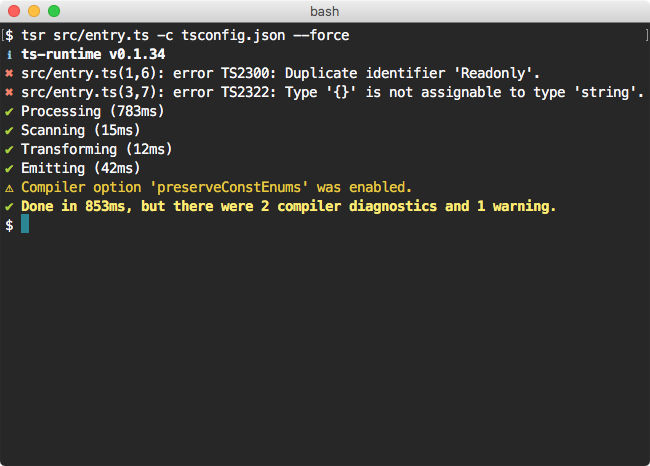
\includegraphics[width=0.75\textwidth]{cli}
\caption{Output of the command line interface, with compiler errors and warnings. The TypeScript file \texttt{entry.ts} within the directory \texttt{src} was compiled, while the TypeScript compiler options where loaded from \texttt{tsconfig.json}, and the transformation process was not aborted on the occurrence of semantic errors, as the \texttt{force} flag was set.}
\label{fig:cli}
\end{figure}

\subsection{Playground}
\label{sec:usage-playground}

To test and try \emph{ts-runtime} in a browser, a playground was created. It takes advantage of the reflection transformation feature, which does not require an underlying file system. While the playground source is not included in the published package on the npm registry, it can be obtained from the repository on GitHub\footnote{\url{https://github.com/fabiandev/ts-runtime}}, where the source code of the entire thesis project is available. The playground is also served directly from this repository\footnote{\url{https://fabiandev.github.io/ts-runtime/}}, as shown in Figure~\ref{fig:playground}.
\begin{figure}
\centering
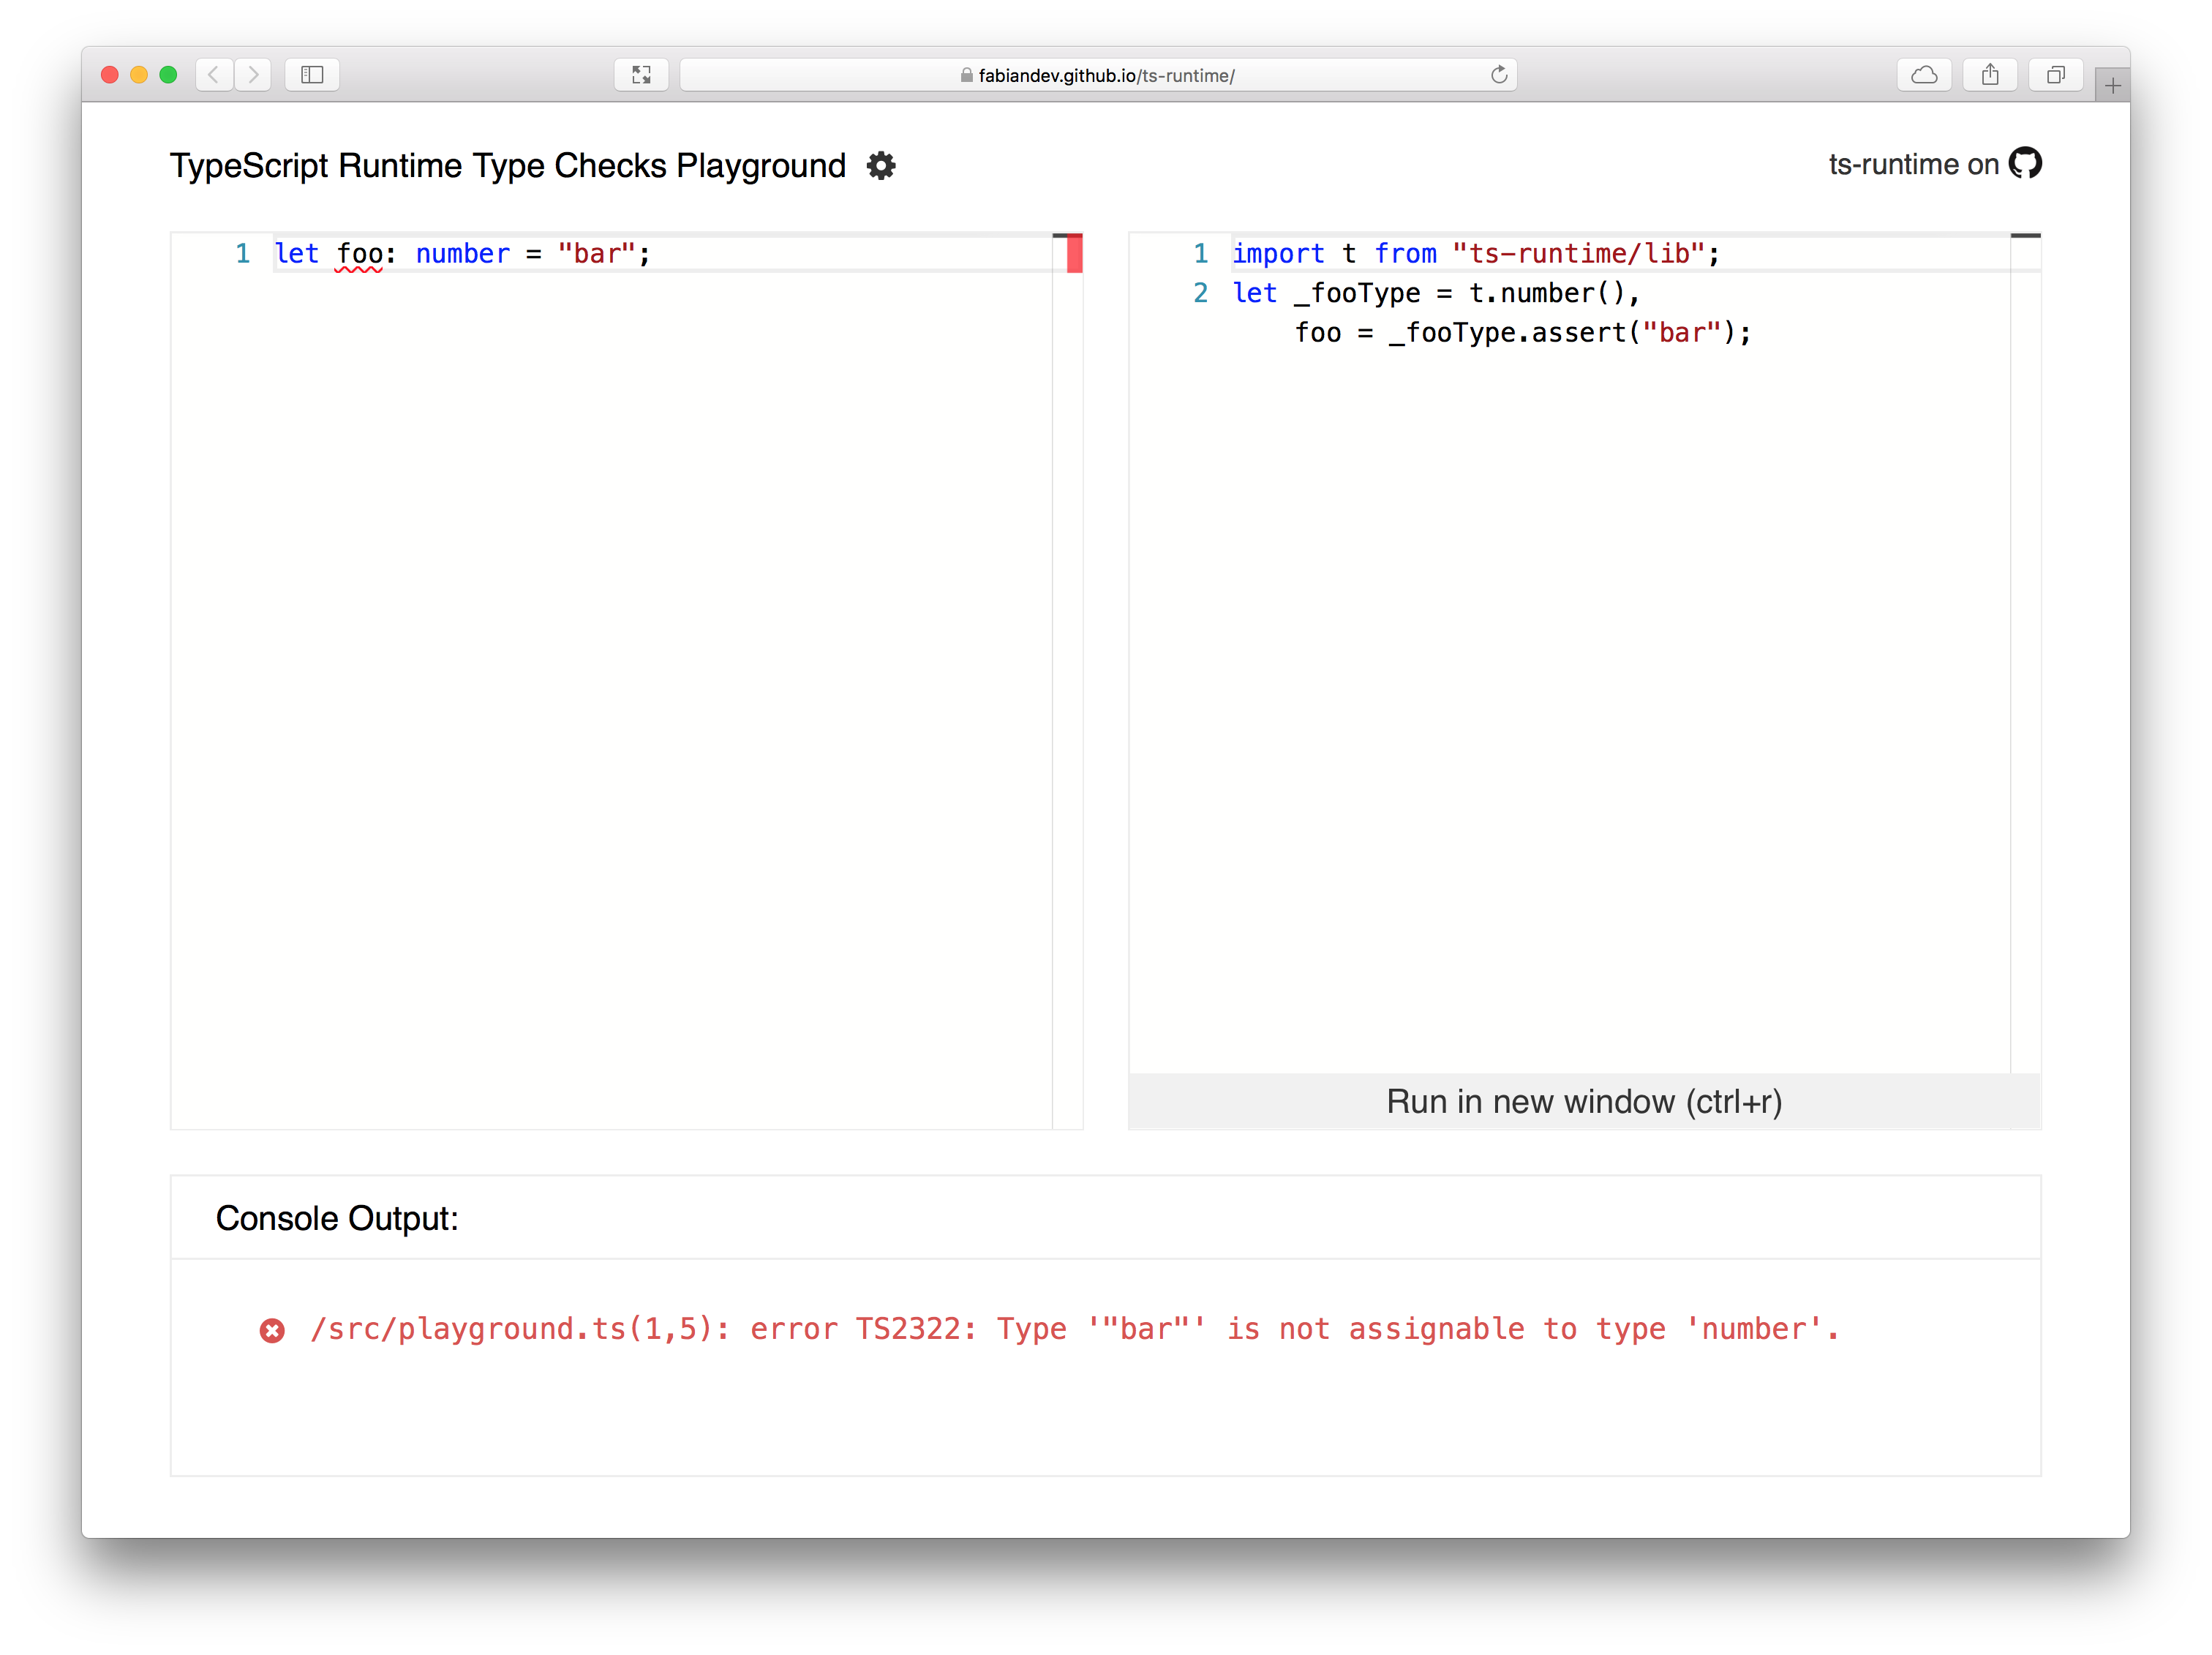
\includegraphics[width=1\textwidth]{playground-shadow}
\caption{Screenshot of the playground of the thesis project, which provides a user interface to test transformations, and its behavior at runtime. Available online at \url{https://fabiandev.github.io/ts-runtime/}.}
\label{fig:playground}
\end{figure}
The transformed and compiled JavaScript code can also be executed in the browser, to not only show the result of the target code, but to also inspect its behavior at runtime.
